%%%%%%%%%%%%  Generated using docx2latex.pythonanywhere.com  %%%%%%%%%%%%%%


\documentclass[a4paper,12pt]{report}

% Other options in place of 'report' are 1)article 2)book 3)letter
% Other options in place of 'a4paper' are 1)a5paper 2)b5paper 3)letterpaper 4)legalpaper 5)executivepaper


 %%%%%%%%%%%%  Include Packages  %%%%%%%%%%%%%%


\usepackage{amsmath}
\usepackage{latexsym}
\usepackage{amsfonts}
\usepackage{amssymb}
\usepackage{graphicx}
\usepackage{txfonts}
\usepackage{wasysym}
\usepackage{enumitem}
\usepackage{adjustbox}
\usepackage{ragged2e}
\usepackage{tabularx}
\usepackage{changepage}
\usepackage{setspace}
\usepackage{hhline}
\usepackage{multicol}
\usepackage{float}
\usepackage{multirow}
\usepackage{makecell}
\usepackage{fancyhdr}
\usepackage[toc,page]{appendix}
\usepackage[utf8]{inputenc}
\usepackage[T1]{fontenc}
\usepackage{hyperref}


 %%%%%%%%%%%%  Define Colors For Hyperlinks  %%%%%%%%%%%%%%


\hypersetup{
colorlinks=true,
linkcolor=blue,
filecolor=magenta,
urlcolor=cyan,
}
\urlstyle{same}


 %%%%%%%%%%%%  Set Depths for Sections  %%%%%%%%%%%%%%

% 1) Section
% 1.1) SubSection
% 1.1.1) SubSubSection
% 1.1.1.1) Paragraph
% 1.1.1.1.1) Subparagraph


\setcounter{tocdepth}{5}
\setcounter{secnumdepth}{5}


 %%%%%%%%%%%%  Set Page Margins  %%%%%%%%%%%%%%


\usepackage[a4paper,bindingoffset=0.2in,headsep=0.5cm,left=1.0in,right=1.0in,bottom=4cm,top=5cm,headheight=5cm]{geometry}
\everymath{\displaystyle}


 %%%%%%%%%%%%  Set Depths for Nested Lists created by \begin{enumerate}  %%%%%%%%%%%%%%


\setlistdepth{9}
\newlist{myEnumerate}{enumerate}{9}
	\setlist[myEnumerate,1]{label=\arabic*)}
	\setlist[myEnumerate,2]{label=\alph*)}
	\setlist[myEnumerate,3]{label=(\roman*)}
	\setlist[myEnumerate,4]{label=(\arabic*)}
	\setlist[myEnumerate,5]{label=(\Alph*)}
	\setlist[myEnumerate,6]{label=(\Roman*)}
	\setlist[myEnumerate,7]{label=\arabic*}
	\setlist[myEnumerate,8]{label=\alph*}
	\setlist[myEnumerate,9]{label=\roman*}

\renewlist{itemize}{itemize}{9}
	\setlist[itemize]{label=$\cdot$}
	\setlist[itemize,1]{label=\textbullet}
	\setlist[itemize,2]{label=$\circ$}
	\setlist[itemize,3]{label=$\ast$}
	\setlist[itemize,4]{label=$\dagger$}
	\setlist[itemize,5]{label=$\triangleright$}
	\setlist[itemize,6]{label=$\bigstar$}
	\setlist[itemize,7]{label=$\blacklozenge$}
	\setlist[itemize,8]{label=$\prime$}



 %%%%%%%%%%%%  Header here  %%%%%%%%%%%%%%


\pagestyle{fancy}
\fancyhf{}
\chead{\vspace{12pt}
\vspace{12pt}
}


 %%%%%%%%%%%%  Footer here  %%%%%%%%%%%%%%


\cfoot{ENF Monitoring Suite – Get-ENFAlertsKyle Timins \par
\vspace{12pt}
ENF Monitoring Suite – Get-ENFAlertsKyle Timins \par
Created 2016Kyle Timins \par
}


 %%%%%%%%%%%%  Print Page Numbers  %%%%%%%%%%%%%%


\rfoot{\thepage}


 %%%%%%%%%%%%  This sets linespacing (verticle gap between Lines) Default=1 %%%%%%%%%%%%%%


\setstretch{1.15}


 %%%%%%%%%%%%  Document Code starts here %%%%%%%%%%%%%%


\title{ENF Alert Emails}
\begin{document}
\maketitle
\sloppy 
 \par


 %%%%%%%%%%%%  This Produces Table Of Contents %%%%%%%%%%%%%%
% Remove \listoffigures if you don't want List of Figures
% Remove \listoftables if you don't want List of Tables


% To be able to get automated contents in these tables
%**********   Properly Follow Styling Guides   ***********

\tableofcontents
\addcontentsline{toc}{chapter}{Contents}
\listoffigures
\addcontentsline{toc}{chapter}{List of Figures}
\listoftables
\addcontentsline{toc}{chapter}{List of Tables}

\begin{flushleft}

 %%%%%%%%%%%%  Start New Page here %%%%%%%%%%%%%%


\newpage

\end{flushleft}\vspace{14pt}
\section*{Get-ENFAlerts}
\addcontentsline{toc}{section}{Get-ENFAlerts}
 \par
The Get-ENFAlerts is a tool used to aggregate and alert when ENFs occur in the specified environments. It has been developed in Powershell v3.0 and JSON. It works in conjunction with configuration files, written in JSON, that are passed in via command line arguments.  \par
\subsection*{Config Files}
\addcontentsline{toc}{subsection}{Config Files}
 \par
The configuration files that are used via this script are written in JSON. JSON is an Object Notation Language created from Javascript. JSON was chosen because it is light weight, easy to parse, and easier to read when compared to XML. If not familiar with JSON, a quick tutorial can be found at the following link: \href{http://www.tutorialspoint.com/json/json $  \_  $ quick $  \_  $ guide.htm}{http://www.tutorialspoint.com/json/json $  \_  $ quick $  \_  $ guide.htm}
 \par
There are two configuration files that are passed into the script: the enfrc and the envrc.  \par
\subsubsection*{enfrc.json}
\addcontentsline{toc}{subsubsection}{enfrc.json}
 \par
The enfrc.json file is the configuration file that is used to define the parameters of the current  $ " $ run $ " $  of the script. This includes what groupings of ENF messages should be looked at, what environments should be looked at, and the configuration of the email that will be sent out. It can be configured to look at multiple environments and/or ENF exception sets so an aggregated list of everything will be sent out. Or it can be configured so there are multiple versions of the configuration file so each only looks at one environment and one set of ENF exception messages, thus creating multiple emails (via multiple runs) that are segmented as to be specific in nature. As a user will tend to end up with a lot of enfrc configuration files, it is recommended to give them proper names, but keep the  $ " $ enfrc.json $ " $  bit at the end to differentiate from the envrc configuration file. \par
By default, the script looks at the first unnamed parameter or the named parameter  $ " $ configFile $ " $ . If no parameter is passed in for the enfrc configuration file, it will default to looking for a file called  $ " $ enfrc.json $ " $  in the same directory level as the Get-ENFAlerts.ps1 file. \par
\paragraph*{Structure and Contents}
\addcontentsline{toc}{paragraph}{Structure and Contents}
 \par
\begin{itemize}
\item \textbf{Output}: This contains the information for the output of the script including files created and the email. It is an object. \par
\begin{itemize}
\item \textbf{File}: This contains the information for the files that can be created from this script. It is an object. \par
\begin{itemize}
\item \textbf{CSV}: Determines if CSV files should be created with data that gets put into the email. It is a Boolean. \par
\item \textbf{JSON}: Determines if JSON files should be created with data that gets put into the email. It is a Boolean. \par
\item \textbf{XML}: Determines if XML files should be created with data that gets put into the email. It is a Boolean. \par
\item \textbf{Zips}: A global on/off switch to determine if the zip files should be downloaded for the Triage ENFs. It is a Boolean. \par
\item \textbf{Suffix}: This is the suffix that will be added to the end of the CSV/JSON/XML files created using this config file. It is a string. \par
\item \textbf{AppendDate}: Determines if a datetime stamp should be added to the folder, in which, the files are saved to, if they are to be saved. It is a Boolean. \par
\item \textbf{Save}: Determines if the CSV/JSON/XML files should be saved to the local disk or if they should be deleted after they have been sent in the email. It is a Boolean. \par
\end{itemize}
\item \textbf{Email}: This is the configuration for the email settings. It is an object. \par
\begin{itemize}
\item \textbf{Subject}: This is the subject of the email that will be sent out. It is static and has no escape characters. It is a string. \par
\item \textbf{Recipient}: This is a hard coded list of recipients for the email. It is an array of objects. \par
\item \textbf{RecipientsScheduled}: This is the way to dynamically add recipients to an email based on a start/end date pair or a service pack. It is an array of objects. \par
\begin{itemize}
\item \textbf{Name}: The name of the person. It is a string. \par
\item \textbf{Email}: The email of the person. It is a string. \par
\item \textbf{ServicePack}: List of service packs that the person should be added to the email. Service packs are counted from Monday to the Friday two weeks ahead. This has priority over the Dates. It is an array of strings. \par
\item \textbf{Dates}: If not using the service pack, the date list holds the start and end dates. It is an array of objects. \par
\begin{itemize}
\item \textbf{StartDate}: The start date of when the user should be added as a recipient. It is a string. \par
\item \textbf{EndDate}: The end date of when the user should be added as a recipient. This has priority over the TimeSpan field. It is a string. \par
\item \textbf{TimeSpan}: The Timespan that the user should be added as a recipient. Use either this or the end date field. The format for this is m/ $  \textbackslash  $ d+[mhd]/ meaning a number followed by 'm' for minutes, 'h' for hours, and 'd' for days. It is a string. \par
\end{itemize}
\end{itemize}
\item \textbf{CC}: This is a hard coded list of carbon copy recipients for the email. It is an array of strings. \par
\item \textbf{Attachment}: Should the CSV, XML, and JSON files be attached to the email. It is a Boolean. \par
\item \textbf{Priority}: What should the priority of the email be? High, normal, or low are the valid entries. \par
\end{itemize}
\end{itemize}
\item \textbf{BaseDir}: This is where all the local files are created and stored, if the settings say so. \par
\item \textbf{ENFSets}: This is the list of ENF sets that the script should check against. It is an array of objects. \par
\begin{itemize}
\item \textbf{Name}: This is the name of the set that will be used by the script. It is a string. \par
\item \textbf{TimeSpan}: This is how long the script should look back for the ENFs in this set. The format for this is m/ $  \textbackslash  $ d+[mhd]/ meaning a number followed by 'm' for minutes, 'h' for hours, and 'd' for days. It is a string. \par
\item \textbf{Zips}: This is how many zips should be downloaded for the set if the setting above says to download the zips. This may become depricated. The format for this is m/ $  \textbackslash  $ d+[fl]/ meaning a number followed by either 'f' for first or 'l' for latest zips. It is a string. \par
\item \textbf{MinCount}: This is the number of occurrence enfs per Triage ENF that should occur before the script will count it the numbers or the email. It is an integer. \par
\item \textbf{Email}: These are the email settings for the ENF set. They determine how the ENF displays on the email. It is an object. \par
\begin{itemize}
\item \textbf{Threshold}: Threshold of how many occurrences are need to occur in the set for it to be added to the email. '0' means always send an email. It is an integer. \par
\item \textbf{Details}: Should~the details section be shown for the ENFs in this set. Contains useful information, but adds bulk to the email.  This controls the whether the rest of the settings in Email matter or not. It is a Boolean. \par
\item \textbf{Stack}: Should the stack be shown in the email section. Can make the email very bulky. It is a Boolean. \par
\item \textbf{OrderBy}: This is the setting to show what order the details section of the email should be ordered in. The valid values are  $ " $ count $ " $  and  $ " $ date $ " $ . Both are descending. \par
\item \textbf{IncludeNotes}: Should the notes on the ENF be shown in the email. These are the notes that are added to the ENF in the ENF tool. It is a Boolean. \par
\item \textbf{IncludeEmptyNotes}: Should there be an empty section for the recipients to add their notes to. This may be depricated. It is a Boolean. \par
\item \textbf{IncludeLatestInfo}: Should there be information in the details section for the latest occurrence. It is a Boolean. \par
\end{itemize}
\item \textbf{ExMsgs}: List of exception messages that should be looked at by the script for this set. It is an array of strings. \par
\item \textbf{NotExMsgs}: List of exception messages that should not be looked at by the script for this set. It is an array of strings. \par
\end{itemize}
\item \textbf{ENFPortfolio}: This is the portfolio that the script should narrow the search to. Used for Daily Builds LOB teams. It is an array of strings. \par
\item \textbf{ENFSkippedPortfolio}: This is the set of portfolios that the script should skip when running it’s search. It is an array of strings. \par
\item \textbf{ENFSkippedStatuses}: This is the list of status of an ENF that should be skipped when getting the list of ENFs. It is an array of strings. \par
\item \textbf{Envs}: This is the environments that should be looked at for each ENFSet. It is an array of objects. \par
\begin{itemize}
\item \textbf{Client}: This is the client of the environment. The spelling and correct values is determined by the environmental configuration file. It is a string. \par
\item \textbf{Env}: This is the environment within the client. The spelling and correct values are determined by the environmental configuration file. It is a string. \par
\end{itemize}
\end{itemize}
\subsubsection*{envrc.json}
\addcontentsline{toc}{subsubsection}{envrc.json}
 \par
The envrc.json file is the environmental configuration file that is used to define the environment that the script is running in. It includes info like the ENF Database server, the SMTP server, the list of valid clients with their environments (and the ENF database tables that store their ENFs), and the conversion from Service Packs to weeks. This configuration will most likely not change between different  $ " $ runs $ " $ , so it is mostly safe to keep one with just the name  $ " $ envrc.json $ " $ . If more are needed, keep the  $ " $ envrc.json $ " $  bit at the end to differentiate from the enfrc configuration file. \par
By default, the script looks at the third unnamed parameter or the named parameter  $ " $ envConfigFile $ " $ . If no parameter is passed in for the envrc configuration file, it will default to looking for a file called  $ " $ envrc.json $ " $  in the same directory level as the GetENFAlerts.ps1 file. \par
\paragraph*{Structure and Contents}
\addcontentsline{toc}{paragraph}{Structure and Contents}
 \par
\begin{itemize}
\item \textbf{ServicePacks}: This is a list of service packs with their start and end dates. It is used in the script to determine if a scheduled recipient should be added to the recipients or not for a desired alert. It is an array of objects. \par
\begin{itemize}
\item \textbf{Release}: Service pack release name. It is a string. \par
\item \textbf{StartDate}: The start date of the service pack. This is the Sunday of the first week. It is a string. \par
\item \textbf{EndDate}: The end date for the service pack. This is the Saturday of the second week. It is a string. \par
\end{itemize}
\item \textbf{ENVLookup}: This is the list of clients with their valid environments and what SQL database to look at. It is an array of objects. \par
\begin{itemize}
\item \textbf{Client}: This is the name of the client. It is a string. \par
\item \textbf{ENVs}: This is a list of environments the client has and what SQL database to look at. It is an array of objects. \par
\begin{itemize}
\item \textbf{Name}: This is the environment that the client has. It is a string. \par
\item \textbf{SQLDB}: This is the SQL database in the ENF SQL Server to look at for the ENFs. It is a string. \par
\end{itemize}
\end{itemize}
\item \textbf{DBServer}: This is the SQL Database server to use in the DB lookups. It is a string. \par
\item \textbf{SMTPServer}: This is the SMTP server to use when sending the email. It is a string. \par
\end{itemize}
\subsubsection*{How to Set Up and Customize the Configuration Files}
\addcontentsline{toc}{subsubsection}{How to Set Up and Customize the Configuration Files}
 \par
This section will show how to set up the enfrc configuration file for a customized run. \textit{The Bare Essentials} will show the most minimalized setup needed to be ready to run the script. The \textit{Full Script Configuration} will show most of the different configurations that are possible to completely customize the enfrc configuration file. See above section, \href{}{Structure and Contents}
, for more information on the enfrc configuration file is structured and what it contains. Note: This section is only about customizing the enfrc configuration file. It does not cover running the script or setting up Scheduled Tasks. These are explained in \href{}{Running Get-ENFAlerts.ps1}
 and \href{}{How to Run Get-ENFAlerts.ps1 via Scheduled Tasks}
. \par
\paragraph*{The Bare Essentials}
\addcontentsline{toc}{paragraph}{The Bare Essentials}
 \par
This section will show what the bare, minimal essentials are needed to set up the enfrc configuration file for customized run. \par
\begin{itemize}
\item What LOBs should the script match against? \par
\begin{itemize}
\item These are put in the  $ " $ ENFLOBs $ " $  section, which is a comma separated array. The LOB codes should be the two letter codes that are used in the ENF tool for the Line of Business. (Should be the same codes that are used in Policy Decisions.) E.g.  $ " $ GL $ " $ ,  $ " $ PF $ " $ ,… \par
\end{itemize}
\item Who should be the recipients and the CC recipients? \par
\begin{itemize}
\item Recipients are put in a comma separated array under \textit{Output.Email.Recipient}. By default, the email address associated with the account used to run the script will be automatically added to the Recipients array when it sends out the email. \par
\item Carbon Copy Recipients are put in a comma separated array under \textit{Output.Email.CC}. \par
\end{itemize}
\item What Exception message(s) should the script compare against? \par
\begin{itemize}
\item By default, the script comes with an ENF set that looks against the Exception Message  $ " $  $  \%  $  $ " $ . This means  $ " $ match any and every exception message $ " $ . Unless specificity is needed, this should be sufficient for running this script. These are stated in a comma separated array under \textit{ENFSets}\textit{. $  \_  $ object $  \_  $ .}\textit{ExMsgs}. \par
\end{itemize}
\item What ENF statuses should be skipped? \par
\begin{itemize}
\item By default, the script will skip  $ " $ Deferred $ " $ ,  $ " $ Environmental $ " $ ,  $ " $ Resolved $ " $ , and  $ " $ In Progress $ " $ . If desired, In Progress may be removed from the list to show any ENFs that have this status. It is not recommended to remove any of the other three statuses as they are meant to remove the ENFs from view. These are stated in a comma separated array under \textit{ENFSkippedStatuses}. \par
\end{itemize}
\item What Client and Environments should the script look at? \par
\begin{itemize}
\item By default, the script is setup to look at DailyBuilds (Prod), Allstate (Prod), and Allstate (QA). If running for Daily Builds only, it is recommended that the two references for Allstate are removed. The valid Client/Environment pairs are specified in the envrc.json configuration file. These are stated in \textit{Envs}\textit{. $  \_  $ object $  \_  $ }. \par
\end{itemize}
\item What should the threshold of ENF occurrences be?  \par
\begin{itemize}
\item The threshold is the number of ENF occurrences in an ENF set that need to happen in the given timespan before an email is sent out. A threshold of 0 means always sends an email, even if there are no occurrences. A threshold of 1 or more means send an email, only if the total number of ENF occurrences in the set is equal to or greater than the threshold. By default, the threshold is set to 1. This can be found under \textit{ENFSets}\textit{. $  \_  $ object $  \_  $ .}\textit{Email.Threshold}. \par
\end{itemize}
\item What time frame should be looked back at? \par
\begin{itemize}
\item By default, the script is setup to look back two hours for the ENF set. This is great for monitoring emergency issues, but for standard use, it is recommended to look back between one day and seven days. (Or one hundred days for the exteme.) It is recommended that the run at the end of the week should look back over the entire week, if not further. And possibly overlapping any daily or every X number of days. (Like running thirty hours back instead of one day/twenty-four hours.) This is because there can be a delay between the error occurring and the ENF being created.  \par
\end{itemize}
\end{itemize}
\paragraph*{Full Script Configuration}
\addcontentsline{toc}{paragraph}{Full Script Configuration}
 \par
Please see the default enfrc.json and envrc.json files to see the full extent of the customizability of the configuration files for this script. \par
\subsection*{The Script}
\addcontentsline{toc}{subsection}{The Script}
 \par
The Get-ENFAlerts.ps1 script is the main tool for this as it contains the code of the program. It is built upon Powershell v3 and.Net technology. As such, .Net 3.5 and Powershell v3 must be installed on the machine prior to running the script.  \par
\subsubsection*{Parameters}
\addcontentsline{toc}{subsubsection}{Parameters}
 \par
The script takes in four optional parameters: \par
\begin{itemize}
\item enfrc.json configuration file \par
\item Starting directory \par
\item envrc.json configuration file \par
\item Validate only switch. \par
\end{itemize}
The configuration files are explained above.  \par
The Starting directory defines the starting directory where the paths for the configuration files will be found. The starting directory can be used if running from a tool like  $ " $ Task Scheduler $ " $  as it will start the powershell instance in  $ " $ C: $  \textbackslash  $ Windows $  \textbackslash  $ System32 $ " $ . Or it can be used if the script is run from a different directory as the config files. \par
The Validate Only switch can be used to make sure that the configuration files are in the right format. It will not run any database lookups or send the email; it will only validate the two configuration files. It is recommended that this option be run after any changes to the configuration files. \par
\subsubsection*{Functionality}
\addcontentsline{toc}{subsubsection}{Functionality}
 \par
The script follows a set procedure in how it works and can be understood by that. This is the process in which the script works: \par
\begin{myEnumerate}
\item The enfrc and envrc files are passed into the script when it is run. \par
\item The script processes the config files and turns them into smaller object that it uses to hold the configuration information for each part. \par
\item The Base Directory and other high level variables are set. \par
\item Foreach ENF set that is in the configuration file: \par
\begin{myEnumerate}
\item It creates an object for that set. \par
\item It goes out and gets a list of Triage ENFs that have occurred within the specified parameters of the set. \par
\item Foreach of the Triage ENFs the last section returned: \par
\begin{myEnumerate}
\item It goes out and gets the latest occurrence information for the ENF \par
\item It goes and gets the occurrence count for the Triage ENF within the time frame supplied. \par
\item An object is created with the information about the Triage ENF, including the occurrence information. This object is then added to the ENF Set object. \par
\item It is determined if the mail threshold has been fulfilled to determine if an email should be sent. \par
\end{myEnumerate}
\item If the mail threshold has not be fulfilled, it checks to see if it should be sending an email based on the threshold being set to 0. \par
\item Add Set object to an  $ " $ Outset $ " $  array. \par
\end{myEnumerate}
\item If specified by the configuration file states, the CSV, XML, and/or the JSON files are created and saved to the working directory within the Base Directory. \par
\item The Email is created by going through the sets. \par
\begin{myEnumerate}
\item The email is only created and sent if the threshold is reached or the threshold for the set is set to 0. \par
\item The summary section is created to give a high level overview. \par
\item The details section is then created to show more in-depth detail about each ENF. \par
\item The script goes through the working directory to add any attachments to the email that have been created. \par
\item The email is then sent. \par
\end{myEnumerate}
\item If the files are set to be saved, the files are then moved to their permanent place in the Base Directory. Else, the files are deleted from the working directory. \par
\end{myEnumerate}
\subsubsection*{Output}
\addcontentsline{toc}{subsubsection}{Output}
 \par
There are three types of outputs that can be created by this script: the email, output files, and zip files. \par
\paragraph*{The Email}
\addcontentsline{toc}{paragraph}{The Email}
 \par
The ENF Alert Message is structured into three main parts: The Summary, the Details, and the Attachments. \par
\subparagraph*{Summary}
\addcontentsline{toc}{subparagraph}{Summary}
 \par
The Summary section is a main overview of the ENFs. It includes the environment (ENV) and the ENF set (Set) for that environment. Within each pair, there is a line that states the time length, total occurrences, and number of Triage ENFs for each pair. It also includes the exception message for that pair. (‘ $  \%  $ ’ means that all exception messages are included.)  The ENV and Set lines are hyperlinks that will take you to that pair’s Details section. (This works in Outlook on the computer, but will not work on a mobile phone.) Here is an example of a summary with two ENVs and one Set per ENV. \par


 %%%%%%%%%%%%  Figure/Image No:1 here %%%%%%%%%%%%%%


\begin{figure}[H]
\begin{center}
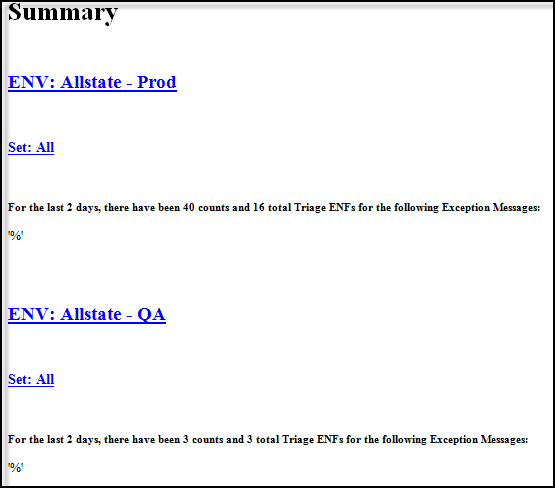
\includegraphics[width=5.78in,height=5.08in]{./uploads_new/ENF_Alert_Emails.docx_DIR/media/image1.png}
\end{center}
\caption{Figure  - Example Summary Section}
\end{figure}


 %%%%%%%%%%%%  Figure/Image No:1 Ends Here %%%%%%%%%%%%%%


\vspace{12pt}
 \par
\subparagraph*{Details}
\addcontentsline{toc}{subparagraph}{Details}
 \par
The Details section is also split up into ENV and Set pair. The pairs show the ENV and the Set, along with a line saying how long of a time period was looked at. (As stated above, clicking the Summary ENV or Set name will bring you to its equivalent in the details section.) This section has a table for each Triage ENF for that Pair. This section has the majority of the needed information on the ENF including the GUID, Counts, ENF Status, CSR (if applicable), Exception Message, Stack Trace (if applicable), ENF notes (if applicable), information about the last occurrence, and a link to the latest zip file. (Note: the link to the latest zip file will only work if you are on Insurity’s network.) The ENF Notes section will only show if the ENF contains notes in the database/tool.  \par
Here is what a pair header looks like: \par


 %%%%%%%%%%%%  Figure/Image No:2 here %%%%%%%%%%%%%%


\begin{figure}[H]
\begin{center}
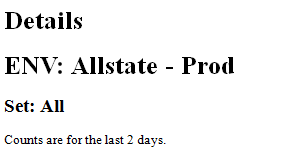
\includegraphics[width=2.99in,height=1.58in]{./uploads_new/ENF_Alert_Emails.docx_DIR/media/image2.png}
\end{center}
\end{figure}


 %%%%%%%%%%%%  Figure/Image No:2 Ends Here %%%%%%%%%%%%%%


\vspace{12pt}
Here are some examples of what the Details grid might look like: \par


 %%%%%%%%%%%%  Figure/Image No:3 here %%%%%%%%%%%%%%


\begin{figure}[H]
\begin{center}
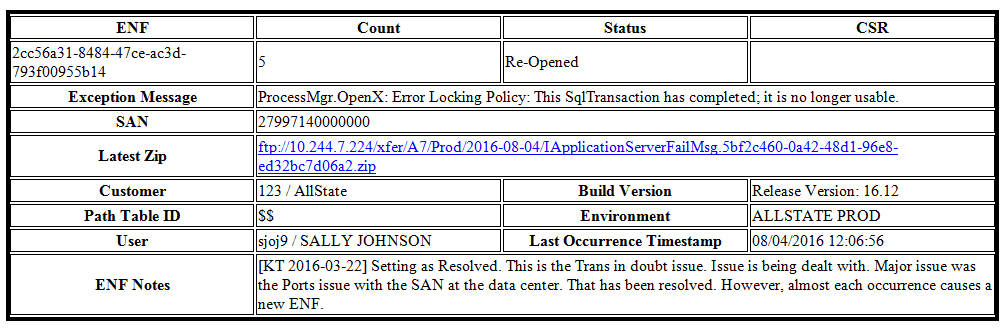
\includegraphics[width=6.5in,height=2.13in]{./uploads_new/ENF_Alert_Emails.docx_DIR/media/image3.png}
\end{center}
\caption{Figure  - Example Details grid with occurrence information}
\end{figure}


 %%%%%%%%%%%%  Figure/Image No:3 Ends Here %%%%%%%%%%%%%%


\vspace{12pt}
 \par


 %%%%%%%%%%%%  Figure/Image No:4 here %%%%%%%%%%%%%%


\begin{figure}[H]
\begin{center}
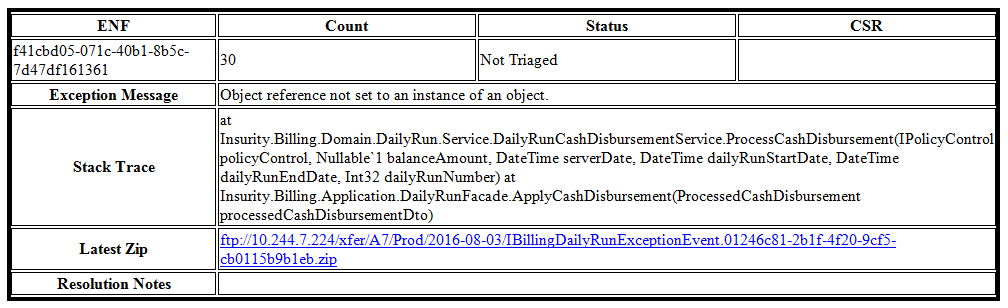
\includegraphics[width=6.5in,height=1.99in]{./uploads_new/ENF_Alert_Emails.docx_DIR/media/image4.png}
\end{center}
\caption{Figure  - Example Details Grid with minimal information}
\end{figure}


 %%%%%%%%%%%%  Figure/Image No:4 Ends Here %%%%%%%%%%%%%%


\vspace{12pt}
 \par


 %%%%%%%%%%%%  Figure/Image No:5 here %%%%%%%%%%%%%%


\begin{figure}[H]
\begin{center}
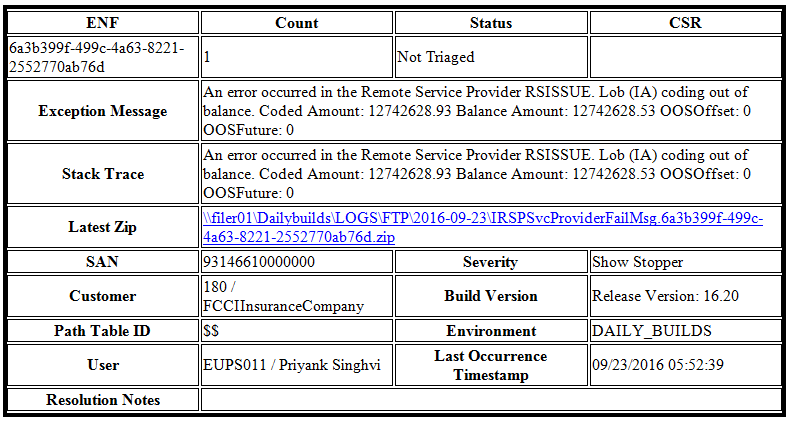
\includegraphics[width=6.5in,height=3.47in]{./uploads_new/ENF_Alert_Emails.docx_DIR/media/image5.png}
\end{center}
\caption{Figure  - Example Detail Grid with a CSR}
\end{figure}


 %%%%%%%%%%%%  Figure/Image No:5 Ends Here %%%%%%%%%%%%%%


\vspace{12pt}
 \par
\vspace{12pt}
\subparagraph*{Attachments}
\addcontentsline{toc}{subparagraph}{Attachments}
 \par
\vspace{12pt}
The last section is the attachments. This contains CSV, XML, and JSON files with the information included in the Details section. But can be parsed via an automated tool (if desired) or used in reports. The default title is formatted as:  $ " $ ENV-Set---Suffix $ " $ , where  $ " $ Set $ " $  is the Client and name of the ENF set and  $ " $ Suffix $ " $  is the name of the group. (Such as  $ " $ Property $ " $  for the Property team.) For example, a title might be  $ " $ DailyBuilds-Prod-All---Property.csv $ " $ . These can be changed if desired. Here is an example of the information, and what it looks like, in the CSV file. \par


 %%%%%%%%%%%%  Figure/Image No:6 here %%%%%%%%%%%%%%


\begin{figure}[H]
\begin{center}
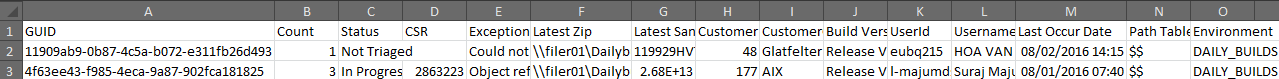
\includegraphics[width=6.5in,height=0.4in]{./uploads_new/ENF_Alert_Emails.docx_DIR/media/image6.png}
\end{center}
\caption{Figure  - An Example CSV file}
\end{figure}


 %%%%%%%%%%%%  Figure/Image No:6 Ends Here %%%%%%%%%%%%%%


\vspace{12pt}
 \par
\paragraph*{The Output Files}
\addcontentsline{toc}{paragraph}{The Output Files}
 \par
As mentioned in the Email section, there are some files that are created by the script that can be emailed or saved to disk. These files contain all the relevant information on the ENFs, but in different forms. The output file types are CSV, XML, and JSON. They all contain the same information, but gives the user the ability to get the info in different formats for what they may need them for. This allows the user to run automated reports on the ENF data without having to transform the data into another format. \par
The creation of these files are determined by Boolean flags in the File.Output section of the enfrc configuration file. As well, that section contains a Boolean value to determine if the files are saved to the computer or if they are deleted after the email is sent. \par
If the files are to be saved on the computer, they will be saved under a folder created in the Base Directory that is defined in the enfrc configuration file. \par
\paragraph*{The Zip Files}
\addcontentsline{toc}{paragraph}{The Zip Files}
 \par
The zip files are the ENF zips that are created when an ENF is registered in the system. They include information including the logs, XML messages, polprints, and other useful information. By default, a link to the latest zip is included in the output files and the details section of the email. However, this option allows for the downloading of multiple zips per ENF to the computer. However, due to the size of these files, they are not sent in the email. So it is recommended to only download the zip files if the script is run on a local machine. \par
There is a  $ " $ master $ " $  Boolean switch in the Output.File section of the enfrc configuration file that controls whether any zips will be downloaded. Then in each of the ENFsets, there is a field to tell the system how many zips should be downloaded per ENF in the set and whether they should from the latest occurrences or the first occurrences. \par
\section*{How to Set Up Powershell}
\addcontentsline{toc}{section}{How to Set Up Powershell}
 \par
If you have not used Powershell before, this is a quick tutorial on how to setup Powershell to be used to run the Get-ENFAlerts script. \par
\subsection*{Upgrading to Powershell v3}
\addcontentsline{toc}{subsection}{Upgrading to Powershell v3}
 \par
By default, Windows 7 comes with Powershell v2 installed on the machine. It needs to be upgraded to version three to work with the Get-ENFAlerts script. \par
\begin{myEnumerate}
\item Ensure that you have Microsoft .NET Framework 4 or higher installed on your machine. If you don’t, you can download .NET Framework 4 from the following Microsoft link. Or you can download the latest version of .NET Framework from Microsoft. \par
\begin{myEnumerate}
\item \href{https://www.microsoft.com/en-us/download/details.aspx?id=17851}{https://www.microsoft.com/en-us/download/details.aspx?id=17851}
 \par
\end{myEnumerate}
\item Download and install the Windows Management Framework 3.0 (i.e. Powershell v3). It can be found at the following link. Make sure you pick the correct architecture for your computer (x86 vs x64). \par
\begin{myEnumerate}
\item \href{https://www.microsoft.com/en-us/download/details.aspx?id=345950x0}{https://www.microsoft.com/en-us/download/details.aspx?id=345950x0}
 \par
\end{myEnumerate}
\item After you have installed both of these, restart your machine.  \par
\item After you have restarted, open a Powershell window and type the following into the window  $ " $  $  \$  $ PSVersionTable $ " $  and hit enter. The output should show  $ " $ PSVersion $ " $  being set to 3.0. \par
\end{myEnumerate}
\subsection*{How to Setup the Profile file}
\addcontentsline{toc}{subsection}{How to Setup the Profile file}
 \par
\subsubsection*{Execution Policy}
\addcontentsline{toc}{subsubsection}{Execution Policy}
 \par
To run scripts in Powershell, the execution policy must be changed. The execution policy determines what scripts can be run on Powershell based on where they originated from and whether they are signed. There are five main execution policies: \par
\begin{itemize}
\item Restricted: Does not load configuration files or run scripts. This is the default setting. \par
\item AllSigned: Requires that any and all scripts and configuration files be signed by a trusted publisher, even if the script was written on the computer running it. \par
\item RemoteSigned: Requires that all scripts and configuration files that have been downloaded from the internet be signed by a trusted publisher. All scripts written on that specific machine can be run on that machine without signing the script. \par
\item Unrestricted: Loads all configuration files and runs all scripts, no matter their origin. If running an unsigned script downloaded from the internet, you will be prompted for permission before running it. \par
\item Bypass: Nothing is blocked and there are no warnings or prompts. \par
\end{itemize}
\subsubsection*{Setting Execution Policy in the Profile}
\addcontentsline{toc}{subsubsection}{Setting Execution Policy in the Profile}
 \par
For the sake of running the Get-ENFAlerts script, we are using either RemoteSigned or Unrestricted. (Substitute Unrestricted for RemoteSigned in the following if you prefer to use that. This just means you will need to add the certificate to your computer and ensure the script is signed before you run it.) \par
\begin{myEnumerate}
\item Open Powershell as Administrator. \par
\item Type the following, sans quotes, into the Powershell window and hit enter. If it prompts you, type  $ " $ y $ " $  and hit enter. \par
{\fontsize{9pt}{9pt}\selectfont Set-ExecutionPolicy Unrestricted} \par
\item Type the following, sans quotes, into the Powershell window and hit enter. \par
\begin{myEnumerate}
\item  $ " $ New-item~–type file –force   $  \$  $ profile $ " $  \par
\end{myEnumerate}
\item Type the following, sans quotes, into the Powershell window and hit enter. An instance of notepad should open. \par
\begin{myEnumerate}
\item  $ " $ Notepad  $  \$  $ profile $ " $  \par
\end{myEnumerate}
\item Put the following lines into the file as the first three lines and save the file. (Type them. Do not copy and paste.) Close out notepad. \par
{\fontsize{9pt}{9pt}\selectfont Set-ExecutionPolicy Unrestricted} \par
{\fontsize{9pt}{9pt}\selectfont  $  \$  $ ProfileRoot = (Split-Path –Parent  $  \$  $ MyInvocation.MyCommand.Path)} \par
{\fontsize{9pt}{9pt}\selectfont  $  \$  $ env:path +=  $ " $ ; $  \$  $ ProfileRoot $ " $ } \par
\item In the Powershell window, type  $ " $ .  $  \$  $ profile $ " $ . There should be no errors. \par
\end{myEnumerate}
\subsection*{How to Import Certificates}
\addcontentsline{toc}{subsection}{How to Import Certificates}
 \par
Depending on the Execution Policy of the machine, the script may need to be signed. This means that the creator uses a certificate to sign the script with a cryptographic signature at the bottom of the script. It is to show that the script has not been modified since it was signed to avoid tampering and malicious code being added. If the script is signed, the public certificate must be added to the computer’s certificate store so that it can validate that the signed script is, indeed, correct. This is only needed on an Execution Policy of AllSigned or RemoteSigned. Unretricted or Bypass do not need a script to be signed. \par
The certificate for any scripts created by Kyle Timins can be found at  $ " $ \href{file:/// $  \textbackslash  $  $  \textbackslash  $ Hfdktiminsw7d $  \textbackslash  $ ENF $  \_  $ Scripts $  \textbackslash  $ PS $  \_  $ TiminsKy $  \_  $ Trusted $  \_  $ Root $  \_  $ Cert.cer}{ $  \textbackslash  $  $  \textbackslash  $ Hfdktiminsw7d $  \textbackslash  $ ENF $  \_  $ Scripts $  \textbackslash  $ PS $  \_  $ TiminsKy $  \_  $ Trusted $  \_  $ Root $  \_  $ Cert.cer}
 $ " $  \par
\subsubsection*{How to Add a Public Certificate to a Computer’s certificate store}
\addcontentsline{toc}{subsubsection}{How to Add a Public Certificate to a Computer’s certificate store}
 \par
\begin{flushleft}\begin{myEnumerate}
\item Open MMC. This can be done by running  $ " $ mmc.exe $ " $ .\vspace{\baselineskip}


 %%%%%%%%%%%%  Figure/Image No:7 here %%%%%%%%%%%%%%


\begin{figure}[H]
\begin{flushleft}
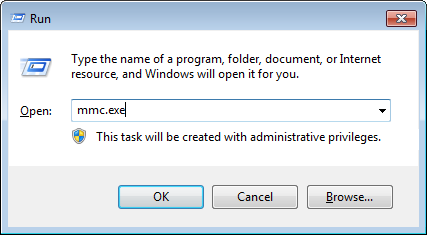
\includegraphics[width=3.22in,height=1.78in]{./uploads_new/ENF_Alert_Emails.docx_DIR/media/image7.png}
\end{flushleft}
\caption{Figure 2-1 - Run MMC.EXE}
\end{figure}


 %%%%%%%%%%%%  Figure/Image No:7 Ends Here %%%%%%%%%%%%%%


\end{flushleft} \par
\end{myEnumerate}
\begin{flushleft}\end{flushleft} \par
\begin{flushleft}\begin{myEnumerate}
\item Click File->Add or Remove Snap-ins\end{flushleft} \par
\begin{flushleft}\item Select  $ " $ Current user $ " $  on the screen and hit  $ " $ OK $ " $ .\end{flushleft} \par
\begin{flushleft}\item Select  $ " $ Certificates $ " $  in the left pane, hit the  $ " $ Add > $ " $  button in the middle. You should now see  $ " $ Certificates – Current User $ " $  in the right pane. Hit  $ " $ OK $ " $ .\vspace{\baselineskip}


 %%%%%%%%%%%%  Figure/Image No:8 here %%%%%%%%%%%%%%


\begin{figure}[H]
\begin{flushleft}
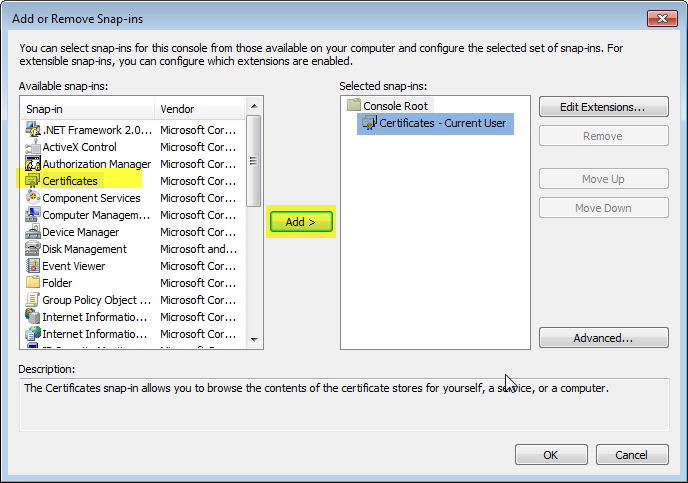
\includegraphics[width=3.22in,height=2.27in]{./uploads_new/ENF_Alert_Emails.docx_DIR/media/image8.png}
\end{flushleft}
\caption{Figure 2-2 - Add Certificates Snap-in}
\end{figure}


 %%%%%%%%%%%%  Figure/Image No:8 Ends Here %%%%%%%%%%%%%%


\end{flushleft} \par
\end{myEnumerate}
\begin{flushleft}\end{flushleft} \par
\begin{flushleft}\begin{myEnumerate}
\item In the left pane, expand  $ " $ Certificates – Current User $ " $ . Then expand  $ " $ Trusted Root Certification Authorities $ " $ . Right click on  $ " $ Certificates $ " $ , and click  $ " $ All Tasks $ " $  then  $ " $ Import $ " $ .\vspace{\baselineskip}


 %%%%%%%%%%%%  Figure/Image No:9 here %%%%%%%%%%%%%%


\begin{figure}[H]
\begin{flushleft}
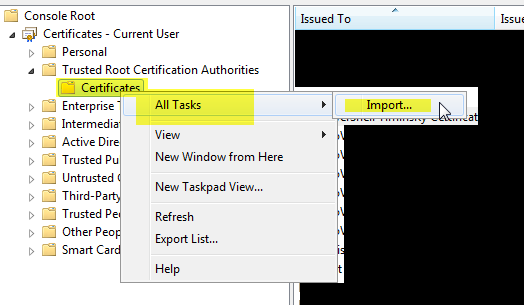
\includegraphics[width=3.28in,height=1.91in]{./uploads_new/ENF_Alert_Emails.docx_DIR/media/image9.png}
\end{flushleft}
\caption{Figure 2-3 - Select Import}
\end{figure}


 %%%%%%%%%%%%  Figure/Image No:9 Ends Here %%%%%%%%%%%%%%


\end{flushleft} \par
\end{myEnumerate}
\begin{flushleft}\end{flushleft} \par
\begin{flushleft}\begin{myEnumerate}
\item In the popup  $ " $ Certificate Import Wizard $ " $ , click  $ " $ Next > $ " $ \vspace{\baselineskip}


 %%%%%%%%%%%%  Figure/Image No:10 here %%%%%%%%%%%%%%


\begin{figure}[H]
\begin{flushleft}
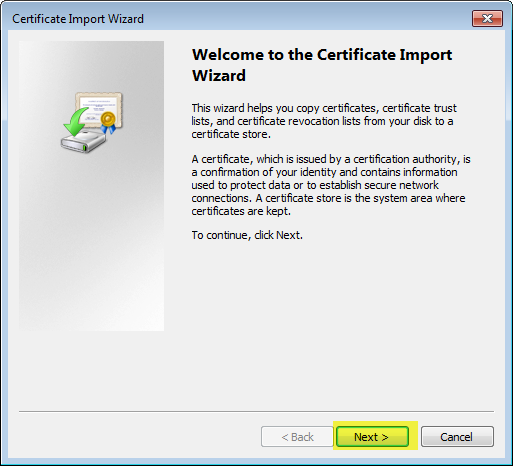
\includegraphics[width=3.28in,height=2.98in]{./uploads_new/ENF_Alert_Emails.docx_DIR/media/image10.png}
\end{flushleft}
\caption{Figure 2-4 - Start Import Process}
\end{figure}


 %%%%%%%%%%%%  Figure/Image No:10 Ends Here %%%%%%%%%%%%%%


\end{flushleft} \par
\end{myEnumerate}
\begin{flushleft}\end{flushleft} \par
\begin{flushleft}\begin{myEnumerate}
\item In the File Name text box, Browse to where you copied the Certificate file.\end{flushleft} \par
\begin{flushleft}\item In the File Name text box, hit  $ " $ Browse $ " $  and select the certificate. Click  $ " $ Next > $ " $ . Example of the box filled after cert has been selected:\vspace{\baselineskip}


 %%%%%%%%%%%%  Figure/Image No:11 here %%%%%%%%%%%%%%


\begin{figure}[H]
\begin{flushleft}
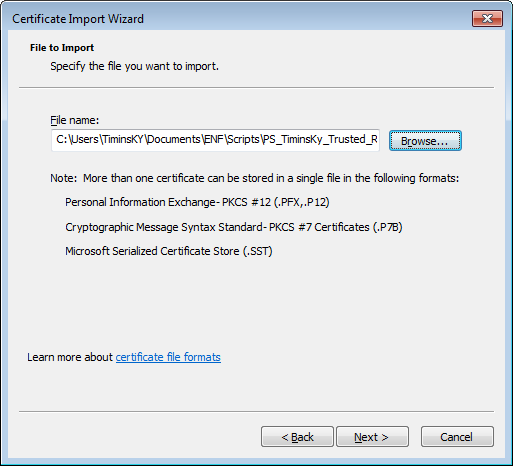
\includegraphics[width=3.24in,height=2.94in]{./uploads_new/ENF_Alert_Emails.docx_DIR/media/image11.png}
\end{flushleft}
\caption{Figure 2-5 - Select Certificate}
\end{figure}


 %%%%%%%%%%%%  Figure/Image No:11 Ends Here %%%%%%%%%%%%%%


\end{flushleft} \par
\end{myEnumerate}
\begin{flushleft}\end{flushleft} \par
\begin{flushleft}\begin{myEnumerate}
\item Click the radio button for  $ " $ Place all certificates in the following store $ " $  and select  $ " $ Trusted Root Certification Authorities $ " $  in the Certificate Store.\vspace{\baselineskip}


 %%%%%%%%%%%%  Figure/Image No:12 here %%%%%%%%%%%%%%


\begin{figure}[H]
\begin{flushleft}
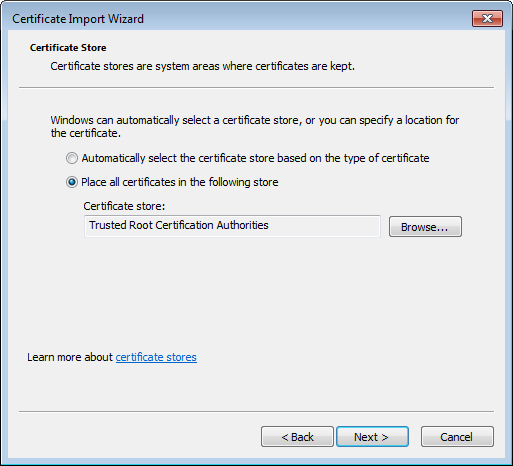
\includegraphics[width=3.32in,height=3.02in]{./uploads_new/ENF_Alert_Emails.docx_DIR/media/image12.png}
\end{flushleft}
\caption{Figure 2-6 - Place in Certificate Store}
\end{figure}


 %%%%%%%%%%%%  Figure/Image No:12 Ends Here %%%%%%%%%%%%%%


\end{flushleft} \par
\end{myEnumerate}
\begin{flushleft}\end{flushleft} \par
\begin{flushleft}\begin{myEnumerate}
\item Hit  $ " $ Next > $ " $  then hit  $ " $ Finish $ " $ .\end{flushleft} \par
\begin{flushleft}\item On the Main MMC screen, you should see  $ " $ PowerShell TiminsKy Certificate Root $ " $  in the list of certificates.\vspace{\baselineskip}


 %%%%%%%%%%%%  Figure/Image No:13 here %%%%%%%%%%%%%%


\begin{figure}[H]
\begin{flushleft}
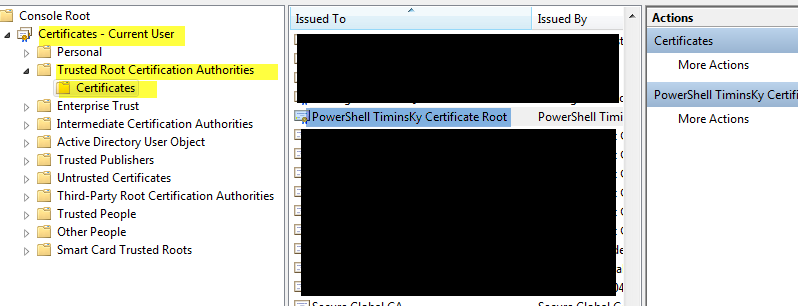
\includegraphics[width=3.25in,height=1.25in]{./uploads_new/ENF_Alert_Emails.docx_DIR/media/image13.png}
\end{flushleft}
\caption{Figure 2-7 - Certificate Added to the Certificate Store}
\end{figure}


 %%%%%%%%%%%%  Figure/Image No:13 Ends Here %%%%%%%%%%%%%%


\end{flushleft} \par
\end{myEnumerate}
\begin{flushleft}\end{flushleft} \par
\begin{flushleft}\begin{myEnumerate}
\item Click  $ " $ File $ " $ -> $ " $ Save $ " $  and save the file. Then exit MMC.\end{flushleft} \par
\begin{flushleft}\item You should now be able to run my scripts.\end{flushleft} \par
\end{myEnumerate}
\subsection*{Running Powershell Scripts}
\addcontentsline{toc}{subsection}{Running Powershell Scripts}
 \par
\subsubsection*{Running Scripts}
\addcontentsline{toc}{subsubsection}{Running Scripts}
 \par
To run a script, you type  $ " $ . $  \textbackslash  $ XXXX.ps1 $ " $  (where XXXX is the name of the script) in the Powershell window (in the directory of the script) and hit enter. \par
\subsubsection*{Getting Help for a Script}
\addcontentsline{toc}{subsubsection}{Getting Help for a Script}
 \par
To get help text for a script, type  $ " $ Get-Help . $  \textbackslash  $ XXXX.ps1 –detailed $ " $  (where XXXX is the name of the script). \par
\subsubsection*{Running Get-ENFAlerts.ps1}
\addcontentsline{toc}{subsubsection}{Running Get-ENFAlerts.ps1}
 \par
\paragraph*{From Powershell}
\addcontentsline{toc}{paragraph}{From Powershell}
 \par
If you are using a file called enfrc.json and envrc.json in the same directory as the Get-ENFAlerts.ps1 file, you can just type  $ " $ . $  \textbackslash  $ Get-ENFAlerts.ps1 $ " $  into the Powershell window and press enter. If you are using a diffenently named configuration file, add the parameter  $ " $ -configFile XXXX $ " $  where XXXX is the name of the configuration file. The same for the environmental configuration file with the parameter  $ " $ -envConfigFile $ " $  \par
For more information on the parameters and the possible ways to use them, type  $ " $ Get-Help . $  \textbackslash  $ Get-ENFAlerts.ps1 -Detailed $ " $  into the Powershell window and press enter. \par
\paragraph*{From Batch Script}
\addcontentsline{toc}{paragraph}{From Batch Script}
 \par
The Get-ENFAlerts.ps1 script can be run from a batch script. It works primarily the same as running from a powershell console, but gives the convenience of double clicking to run. Here is what you would put in the batch script: \par
{\fontsize{9pt}{9pt}\selectfont cd  $ " $ C: $  \textbackslash  $ Directory $  \textbackslash  $ where $  \textbackslash  $ the $  \textbackslash  $ Get-ENFAlerts.ps1 $  \textbackslash  $ script $  \textbackslash  $ resides $ " $ } \par
{\fontsize{9pt}{9pt}\selectfont Powershell . $  \textbackslash  $ Get-ENFAlerts.ps1 –configFile . $  \textbackslash  $ enfrc.json} \par
\subsubsection*{How to Run Get-ENFAlerts.ps1 via Scheduled Tasks}
\addcontentsline{toc}{subsubsection}{How to Run Get-ENFAlerts.ps1 via Scheduled Tasks}
 \par
Setting up a scheduled task to run the Get-ENFAlerts.ps1 script is not a difficult task. The only difference between how the script is run is that the Starting directory field is used. Here are the steps to creating a scheduled task to run the script. \par
\begin{myEnumerate}
\item Open the Start Menu and type  $ " $ Task Scheduler $ " $  into the box. At the top of the output, you should see the link to open the scheduler. \par


 %%%%%%%%%%%%  Figure/Image No:14 here %%%%%%%%%%%%%%


\begin{figure}[H]
\begin{center}
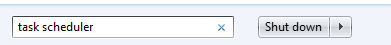
\includegraphics[width=4.07in,height=0.47in]{./uploads_new/ENF_Alert_Emails.docx_DIR/media/image14.png}
\end{center}
\caption{Figure 8 - Start Menu Search}
\end{figure}


 %%%%%%%%%%%%  Figure/Image No:14 Ends Here %%%%%%%%%%%%%%


\vspace{12pt}
\end{myEnumerate}
 \par


 %%%%%%%%%%%%  Figure/Image No:15 here %%%%%%%%%%%%%%


\begin{figure}[H]
\begin{center}
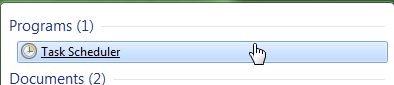
\includegraphics[width=4.1in,height=0.89in]{./uploads_new/ENF_Alert_Emails.docx_DIR/media/image15.png}
\end{center}
\caption{Figure 9 - Start Menu Results}
\end{figure}


 %%%%%%%%%%%%  Figure/Image No:15 Ends Here %%%%%%%%%%%%%%


\vspace{12pt}
 \par
\begin{myEnumerate}
\item On the left hand side of the window, you should see the folder structure of the tasks. Open  $ " $ Task Scheduler Library $ " $  and you should see a folder called  $ " $ User $ " $ . Click this folder. This is where the scheduled tasks will be created. \par


 %%%%%%%%%%%%  Figure/Image No:16 here %%%%%%%%%%%%%%


\begin{figure}[H]
\begin{center}
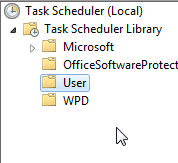
\includegraphics[width=1.85in,height=1.7in]{./uploads_new/ENF_Alert_Emails.docx_DIR/media/image16.png}
\end{center}
\caption{Figure 10 – Task Scheduler Library}
\end{figure}


 %%%%%%%%%%%%  Figure/Image No:16 Ends Here %%%%%%%%%%%%%%


\vspace{12pt}
\end{myEnumerate}
 \par
\begin{myEnumerate}
\item Right click on the User folder and select  $ " $ Create Basic Task $ " $ . (This guide will show how to use the Basic Wizard interface to create a task. If desired, you can simply select  $ " $ Create Task $ " $ . This will give you more control over the task itself, but is less intuitive in how to create a task.) \par
\item In the name field, type in a name that will tell you what the task is. An example would be  $ " $ Daily Builds – ENF Alerts – Daily Run. $ " $  \par
\item In the Description field, you can add more detail so it is more obvious what the task is doing and why it is there. This field is optional. \par
\item Hit the Next button. You will now be on the  $ " $ Trigger $ " $  page. This is how often you want to run the script. (The choices are simplified on this page since it is in the Basic Task Wizard. You will have the option to modify this setting with more granularity after it is created.) After selecting the trigger, hit the Next button. \par
\item If prompted, select the starting time, date, day of the week, month, etc that is shown on this page. This is only if you selected to have the task work on a timed schedule rather than based on a computer event. \par
\item On the Action page, select  $ " $ Start a Program $ " $ . Hit the Next button. \par
\item If using pure Powershell to run the script: \par
\begin{myEnumerate}
\item In the  $ " $ Program/script $ " $  text box, put  $ " $ Powershell.exe $ " $ . \par
\item In the  $ " $ Add Arguments $ " $  section, you are going to add the information on the script itself. \par
\begin{myEnumerate}
\item Here is an example of what it will look like if you use the standard enfrc and envrc (in the same directory as the script) and that directory is  $ " $ C: $  \textbackslash  $ ENF $  \textbackslash  $ Scripts $ " $ . \par
\end{myEnumerate}
\end{myEnumerate}
\end{myEnumerate}
{\fontsize{9pt}{9pt}\selectfont C: $  \textbackslash  $ ENF $  \textbackslash  $ Scripts $  \textbackslash  $ Get-ENFAlerts.ps1  $ " $ enfrc.json $ " $   $ " $ C: $  \textbackslash  $ ENF $  \textbackslash  $ Scripts $ " $ } \par
\begin{myEnumerate}
\item \begin{myEnumerate}
\item \begin{myEnumerate}
\item Here is an example if you are using custom enfrc configuration file in a subfolder called  $ " $ Config $ " $  and the starting directory is  $ " $ C: $  \textbackslash  $ Users $  \textbackslash  $ Timinsky $  \textbackslash  $ scripts $  \textbackslash  $ EnfEmergencyAlerts $ " $  \par
\end{myEnumerate}
\end{myEnumerate}
\end{myEnumerate}
{\fontsize{9pt}{9pt}\selectfont C: $  \textbackslash  $ Users $  \textbackslash  $ TiminsKy $  \textbackslash  $ Scripts $  \textbackslash  $ EnfEmergencyAlerts $  \textbackslash  $ Get-ENFAlerts.ps1  $ " $ Configs $  \textbackslash  $ DailyBuilds-CL-Property-7DayRollup-enfrc.json $ " $   $ " $ C: $  \textbackslash  $ Users $  \textbackslash  $ TiminsKy $  \textbackslash  $ Scripts $  \textbackslash  $ EnfEmergencyAlerts $ " $ } \par
\begin{myEnumerate}
\item If using the Batch script method: \par
\begin{myEnumerate}
\item In the  $ " $ Program/script $ " $  text box, put: \par
\end{myEnumerate}
\end{myEnumerate}
{\fontsize{9pt}{9pt}\selectfont  $ " $ C: $  \textbackslash  $ Location $  \textbackslash  $ of $  \textbackslash  $ the $  \textbackslash  $ batch $  \textbackslash  $ script $  \textbackslash  $ FILE.bat $ " $ } \par
\begin{myEnumerate}
\item Click next and then click save. \par
\item You have created a scheduled task that will run the script at the desired time/frequency.  \par
\end{myEnumerate}
It should be noted that when the script runs, it will pop up a PowerShell window for a couple of seconds and then vanish. This is the way that it is designed to work. \par
\section*{How to Remediate an ENF}
\addcontentsline{toc}{section}{How to Remediate an ENF}
 \par
\subsection*{Determine the Severity of the ENF}
\addcontentsline{toc}{subsection}{Determine the Severity of the ENF}
 \par
While there is a field on the ENF for severity, it is based upon the number of occurrences and is not always a good measure of what the severity actually is. The severity should be determined by the person doing the triage based upon how impactful the error is, how high the count is, and will it impact the end user. These are the factors that should be used if a CSR is created for the ENF. \par
\subsection*{Adding Comments to the ENF}
\addcontentsline{toc}{subsection}{Adding Comments to the ENF}
 \par
Comments on a ENF go in the  $ " $ Comments $ " $  textbox in the  $ " $ Notification Comments $ " $  section at the bottom of the main page. Use Ctrl+Enter to create a new line within the text box. Comments should be presented in a newest to latest order, so any new comments should be added to the top of the comments list. Each comment should be in the following format: \par
{\fontsize{9pt}{9pt}\selectfont [FL YYYY-MM-DD] This is a comment.} \par
Where  $ " $ FL $ " $  is the initials of first and last name,  $ " $ YYYY $ " $  is the year in 4 character format,  $ " $ MM $ " $  is the month in two character format, and  $ " $ DD $ " $  is the day in two character format. An example would be: \par
{\fontsize{9pt}{9pt}\selectfont [KT 2016-08-01] This is an example comment.} \par
\subsection*{Setting the ENF to In Progress}
\addcontentsline{toc}{subsection}{Setting the ENF to In Progress}
 \par
If a CSR is being created for the ENF, then the ENF should be moved to a status of  $ " $ In Progress $ " $ . It should only be in this state if there is a CSR created for it. If no CSR has been created, then keep the ENF in Not Triaged or ReOpened. \par
\subsubsection*{Creating a CSR for the ENF}
\addcontentsline{toc}{subsubsection}{Creating a CSR for the ENF}
 \par
If it is determined that remediation is needed for the ENF, the next step is to create a CSR for the ENF. \par
When creating a CSR for an ENF, a few rules should be used to ensure there is the proper amount of information. \par
\begin{itemize}
\item Client: This should be set to  $ " $ INT $ " $ . Do not set it to the client as they should not be able to see the CSRs we create for ENFs. \par
\item Sub Client: If the error impacts a specific client only, then the client should be added to the Sub Client section. At the moment, there are only a hand full of valid clients in this section, so only add if that client exists in the list. \par
\item Title: The title should start with  $ " $ ENF –  $ " $  to show that the CSR was created due to an internal ENF. \par
\item Detailed Description: On top of the normal information that should be included in the description, ensure that the GUID for the ENF is included in the following format. This is to allow an easy lookup of the ENF in the tool from the CSR. \par
\begin{itemize}
\item GUID  $  \{  $ XXXXXXXXXX-XXXX-XXXX-XXXX-XXXXXXXXXX  $  \}  $  \par
\end{itemize}
\item Detailed Description: It is recommended that the stack trace should be included in the description. The stack trace can be obtained via either the ENF tool, the ENF Alert email, or the email.html found in the ENF zip. \par
\item In the Category field, fill the field with  $ " $ DBENF $ " $ . This is to allow for easy isolation of the Daily Builds ENFs when creating a search in PPM. \par
\item Ensure that that the latest ENF zip from the ENF is attached to the CSR. If possible, more than one is preferable. The link for the latest ENF zip can be found in the details section of the ENF or in the ENF tool. \par
\item It is recommended to attach a polprint of the latest policy on the ENF. This is due to the fact that Daily Builds ENFs do not contain polprints as a way to conserve on drive space. Adding a polprint of the policy as soon after the ENF is created is desired since the policy can be changed after the ENF is created and can make triage  $  \&  $  analysis impossible. \par
\end{itemize}
\subsection*{Setting the ENF to Resolved}
\addcontentsline{toc}{subsection}{Setting the ENF to Resolved}
 \par
If it has been determined that the ENF is a non-issue, then the status should be set to Resolved. Setting an ENF to Resolved should only be done if there is no remediation for the ENF.  \par
As well, any non  $ " $ SS $ " $  ENF should auto resolve from In Progress, Not Triaged, and Re-Opened after 15 days with no occurrences. \par
\section*{ENF Crash Course}
\addcontentsline{toc}{section}{ENF Crash Course}
 \par
\subsection*{ENF Overview – Enterprise Notification Facility}
\addcontentsline{toc}{subsection}{ENF Overview – Enterprise Notification Facility}
 \par
ENF stands for \textit{Enterprise Notification Facility}. On the server side, it is an enterprise level service that standardizes and enhances how application failures are handled. On the user (person triaging) side, it is a collection of information about a crash that occurred within the system. \par
When an error or crash occurs and there is code in the section to create an ENF, the service creates a  $ " $ package $ " $  called an ENF. The package is a zip file that contains information such as stack traces, information overviews, polprints, configuration files, etc. It does a freeze of all these files and contains them in the zip file. Not all information in the zip file will be relevant or useful to the current error at hand. As well, the information is added to a database which stores the information for later retrieval and for use by the ENF utility. (For more information on the database, please see the \href{}{How to Use the ENF Database}
 section.)  \par
In this document, the terms ENF and Triage ENF will be used. And ENF is a collection of information about a specific "crash" that happened. They all have different GUIDS as their primary key. A Triage ENF is the ENF with the first record of a specific Stack trace. All of the specific crash ENFs are assigned these Triage ENF GUIDS and are referred to as occurrences of a Triage ENF. It is a one-to-many relationship. In most cases, only the Triage ENF and its GUID will be what is discussed and the individual ENFs will only be useful for their SANs, Timestamps, and zip files. \par
\subsection*{ENF Utility }
\addcontentsline{toc}{subsection}{ENF Utility }
 \par
The ENF utility is used as a front-end to the ENF database that is built in Microsoft Access. From this tool, you can: view detailed information about an ENF, modify information about an ENF, and view reports of top count ENFs for a certain timeframe. \par
There are three major screen types on the ENF utility: The Unique Notifications Edit screen, the "Reports" style screen, and the "List" style screen. The report and list style screen have multiple variations. For the purposes of this document, the only reports style screens will be TriageTopXAndSSNotifications  $  \&  $  GetTopXAndSSNotifications and the only list style screens will be the GetAllDistinctByStack  $  \&  $  GetAllDistinctBySAN. \par
\subsection*{Unique Notifications Edits}
\addcontentsline{toc}{subsection}{Unique Notifications Edits}
 \par
\vspace{10pt}
The Unique Notifications Edits screen is the main landing screen. It is used to select your connection, select queries, search, and to display information on an ENF. Here is a breakdown of the screen. \par
\vspace{12pt}
\subsubsection*{Top Bar:}
\addcontentsline{toc}{subsubsection}{Top Bar:}
 \par
\begin{flushleft}\begin{itemize}
\item Connection\end{flushleft} \par
\begin{flushleft}\begin{itemize}
\item These are the different environments that you can look at. Most are self-explanatory. The only main note is that AllState $  \_  $ PreProd looks at both AllState QA Environments (PreProd and Test). And DailyBuilds looks at DailyBuilds, the MP0X environments, and the perimeter environments.\end{flushleft} \par
\begin{flushleft}\item After selecting, hit the button to the right of the dropdown.\end{flushleft} \par
\begin{flushleft}\end{itemize}
\item ENF Filter\end{flushleft} \par
\begin{flushleft}\begin{itemize}
\item These are basically a set of parameters that are predefined. For instance, you can select the "Billing Team" filter and it will only show ENFs that have their Portfolio as "Billing".\end{flushleft} \par
\begin{flushleft}\end{itemize}
\item Queries\end{flushleft} \par
\begin{flushleft}\begin{itemize}
\item These are basically different SQL queries that you can run. Most are self-explanatory.\end{flushleft} \par
\begin{flushleft}\begin{itemize}
\item GetAllDistinctByXXXXXXX will get all of the ENFs in the current environment that matches the value in the popup. The result will be on another tab and will display in a spreadsheet format. These search every ENF collected in the database (assuming they have not been deleted).\end{flushleft} \par
\begin{flushleft}\item GetTop5AndSSNotifications will get a list of  $ " $ Top $ " $  ENFs (basically the largest counts) and a list of SS ENFs (Ones that have certain types that are considered more important.) They are grouped by ExceptionDate and ordered by TodaysCount. The popups for this are:\end{flushleft} \par
\begin{flushleft}\begin{itemize}
\item Select a day to look at\end{flushleft} \par
\begin{flushleft}\item How many days to look at. These look at the Month day, so 1 day would include 2015-06-03 and 2015-06-02.\end{flushleft} \par
\begin{flushleft}\item How many top ENFs. We usually look at 20.\end{flushleft} \par
\begin{flushleft}\end{itemize}
\item TriageTopXAndSSNotifications will get a list similar to the GetTop5AndSSNotificiations, but is defaulted to one day and 20 top. As well, it has a mini selection at the top to view and edit select information. It is more convenient than the GetTop5AndSSNotifications for triaging, but loses some information that is important.\end{flushleft} \par
\begin{flushleft}\end{itemize}
\item Hit the button on the right of the dropdown to go to the selected screen.\end{flushleft} \par
\begin{flushleft}\end{itemize}
\item Srch Field  $  \&  $  Srch Txt\end{flushleft} \par
\begin{flushleft}\begin{itemize}
\item This will search the current environment. You select what you want to search by. Most are pretty much self-explanatory. Here are the ones I use the most.\end{flushleft} \par
\begin{flushleft}\begin{itemize}
\item GUID is the triage GUID.\end{flushleft} \par
\begin{flushleft}\begin{itemize}
\item When getting lists from the queries, you would use the Triage GUID with this search to see that ENF.\end{flushleft} \par
\begin{flushleft}\end{itemize}
\item CSR will search all ENFs for ones that contain that CSR.\end{flushleft} \par
\begin{flushleft}\item StackTrace will search for the part of the StackTrace you paste into the txt field. \end{flushleft} \par
\begin{flushleft}\item Exception message is the same as StackTrace but will the Exception Message\end{flushleft} \par
\begin{flushleft}\item SAN will search all of the Triage ENFs' SANs. This is limited to the first SAN reported with the Stack Trace of the Triage ENF. It is better to use GetAllDistinctBySAN as that will search all ENF records instead of only the Triage ENFs.\end{flushleft} \par
\begin{flushleft}\end{itemize}
\item Press the magnifying glass button on the right to search.\end{flushleft} \par
\vspace{12pt}
\end{itemize}
\end{itemize}


 %%%%%%%%%%%%  Figure/Image No:17 here %%%%%%%%%%%%%%


\begin{figure}[H]
\begin{center}
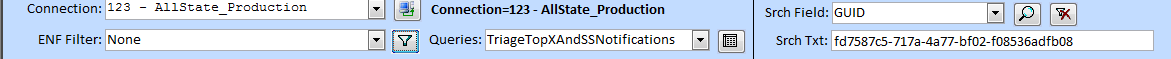
\includegraphics[width=6.5in,height=0.33in]{./uploads_new/ENF_Alert_Emails.docx_DIR/media/image17.png}
\end{center}
\caption{Figure  - The Top Bar of the Main Screen}
\end{figure}


 %%%%%%%%%%%%  Figure/Image No:17 Ends Here %%%%%%%%%%%%%%


\vspace{12pt}
 \par
\subsubsection*{Main Screen}
\addcontentsline{toc}{subsubsection}{Main Screen}
 \par
\begin{flushleft}\begin{itemize}
\item Environment is the environment that they were created in. \end{flushleft} \par
\begin{flushleft}\item Occurrences is the count of occurrences since the LAST Reopen (or open if no reopens.)\end{flushleft} \par
\begin{flushleft}\item Reopens is the number of times the Triage ENF has had a status of Re-Open. \end{flushleft} \par
\begin{flushleft}\item Total Occ is the total number of occurrences since the very first open.\end{flushleft} \par
\begin{flushleft}\item Created Date is the timestamp of the first occurrence of that last Reopen.\end{flushleft} \par
\begin{flushleft}\item Last Date is the timestamp of the last occurrence to happen.\end{flushleft} \par
\begin{flushleft}\item User Email, SAN, PolicyNo, and User Name are from the first occurrence of the enf.\end{flushleft} \par
\begin{flushleft}\item Status\end{flushleft} \par
\begin{flushleft}\begin{itemize}
\item Not triaged: Nothing with the ENF has been done\end{flushleft} \par
\begin{flushleft}\item In Progress: Something is happening with it. A CSR is created. I’ve been using that for when I send emails to people about them.\end{flushleft} \par
\begin{flushleft}\item Resolved: Marking that something is complete. DON’T actually use this. If you set to resolved before the code has shipped back, it will just reopen the ENF.\end{flushleft} \par
\begin{flushleft}\item Re-Opened: Same as Not Triaged, just that the ENF has had an occurrence since it was resolved or auto-resolved.\end{flushleft} \par
\begin{flushleft}\item Auto-Resolved. The system sets the ENF to Auto-resolved after a period of time of no occurrences in 30 days. In Allstates environment, this only happens to TOP ENFs, not to SS ENFs.\end{flushleft} \par
\begin{flushleft}\end{itemize}
\item Severity: Determined by number of occurrences and type.\end{flushleft} \par
\begin{flushleft}\item GUID: The Triage GUID of the ENF collection.\end{flushleft} \par
\begin{flushleft}\item Assigned To and CSR: These you manually enter to store info on the who is working on it and the CSR.\end{flushleft} \par
\begin{flushleft}\item LOB Code: This is what comes through the ENF as the LOB causing the issue. It is usually correct.\end{flushleft} \par
\vspace{12pt}
\end{itemize}


 %%%%%%%%%%%%  Figure/Image No:18 here %%%%%%%%%%%%%%


\begin{figure}[H]
\begin{center}
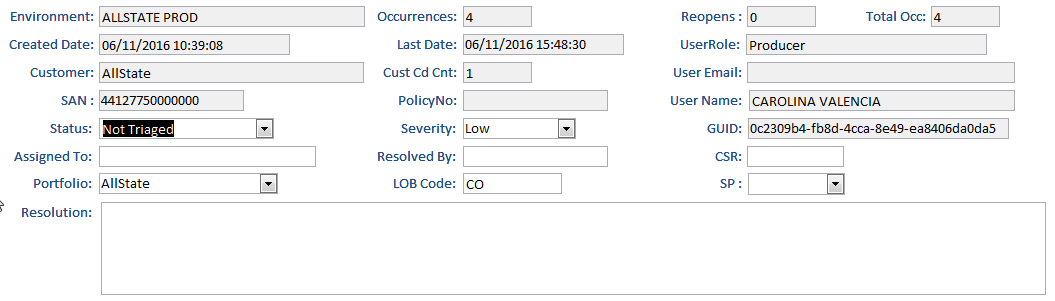
\includegraphics[width=6.5in,height=1.85in]{./uploads_new/ENF_Alert_Emails.docx_DIR/media/image18.png}
\end{center}
\caption{Figure  - Main Section of the Main Screen}
\end{figure}


 %%%%%%%%%%%%  Figure/Image No:18 Ends Here %%%%%%%%%%%%%%


\vspace{12pt}
 \par
\subsubsection*{Original Notification Error Info}
\addcontentsline{toc}{subsubsection}{Original Notification Error Info}
 \par
\begin{flushleft}\begin{itemize}
\item Type is the type of ENF thrown as defined in the code and ServiceBus.\end{flushleft} \par
\begin{flushleft}\item This is the First occurrence information\end{flushleft} \par
\begin{flushleft}\begin{itemize}
\item StackTrace: This is the stack for the error. It is what determines if an occurrence is the same ENF. So all occurrences have the same stack as this section.\end{flushleft} \par
\begin{flushleft}\item Excep Msg: This is the Exception Message. All occurrences have the same exception message as this section.\end{flushleft} \par
\begin{flushleft}\item Zip Pkg: This is the zip for the first occurrence.\end{flushleft} \par
\end{itemize}
\end{itemize}


 %%%%%%%%%%%%  Figure/Image No:19 here %%%%%%%%%%%%%%


\begin{figure}[H]
\begin{center}
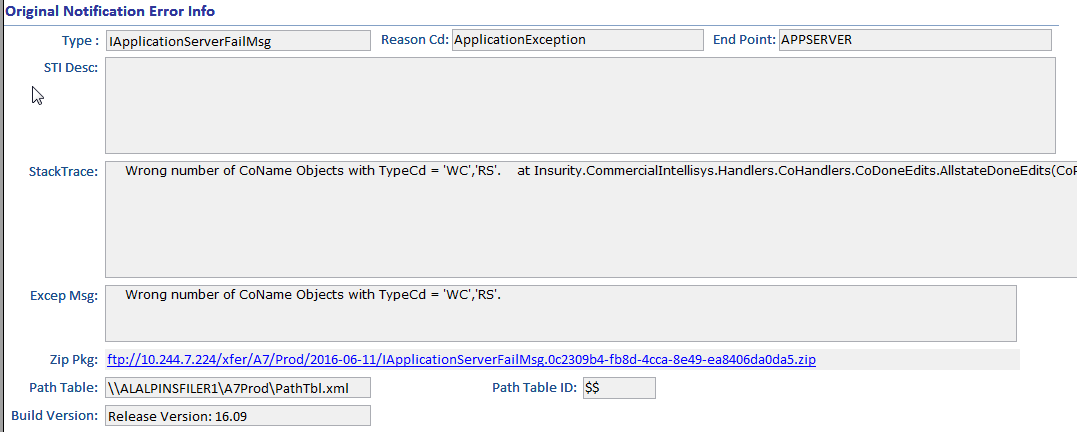
\includegraphics[width=6.5in,height=2.61in]{./uploads_new/ENF_Alert_Emails.docx_DIR/media/image19.png}
\end{center}
\caption{Figure  - Original Notification Information Section of the Main Screen}
\end{figure}


 %%%%%%%%%%%%  Figure/Image No:19 Ends Here %%%%%%%%%%%%%%


\vspace{12pt}
 \par
\vspace{12pt}
\vspace{12pt}
\subsubsection*{Latest Notification Error Info}
\addcontentsline{toc}{subsubsection}{Latest Notification Error Info}
 \par
\begin{flushleft}\begin{itemize}
\item This is the last occurrence.\end{flushleft} \par
\begin{flushleft}\item Environment: The environment of the ENF.\end{flushleft} \par
\end{itemize}


 %%%%%%%%%%%%  Figure/Image No:20 here %%%%%%%%%%%%%%


\begin{figure}[H]
\begin{center}
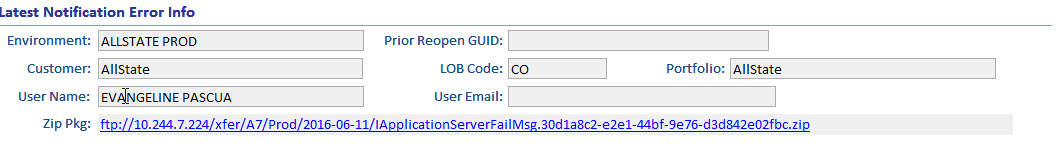
\includegraphics[width=6.5in,height=0.95in]{./uploads_new/ENF_Alert_Emails.docx_DIR/media/image20.png}
\end{center}
\caption{Figure  - Latest Notification Information Section of the Main Screen}
\end{figure}


 %%%%%%%%%%%%  Figure/Image No:20 Ends Here %%%%%%%%%%%%%%


\vspace{12pt}
 \par
\subsubsection*{Notification Comments}
\addcontentsline{toc}{subsubsection}{Notification Comments}
 \par
\begin{flushleft}\begin{itemize}
\item This is where comments about the ENF are put. They are usually prepended with your initials and the date in ISO format (YYYY-MM-DD) all surrounded by square brackets followed by the comment. Use Ctrl+Enter to make a new line.\end{flushleft} \par
\end{itemize}
To save any edits made, you must click the dark grey bar on the left side of the screen. It will get darker after it has been click signaling the save happened. \par


 %%%%%%%%%%%%  Figure/Image No:21 here %%%%%%%%%%%%%%


\begin{figure}[H]
\begin{center}
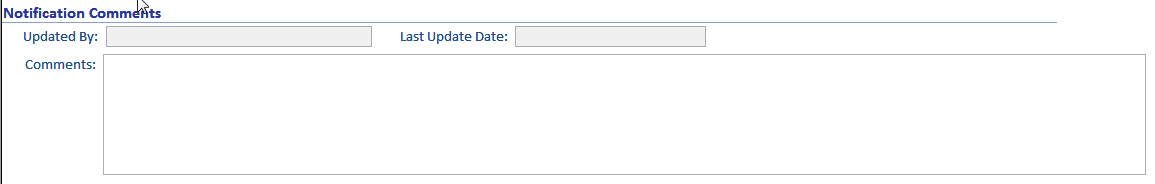
\includegraphics[width=6.5in,height=1.04in]{./uploads_new/ENF_Alert_Emails.docx_DIR/media/image21.png}
\end{center}
\caption{Figure  - Comments Section of the Main Screen}
\end{figure}


 %%%%%%%%%%%%  Figure/Image No:21 Ends Here %%%%%%%%%%%%%%


\vspace{12pt}
 \par
\subsubsection*{Queries}
\addcontentsline{toc}{subsubsection}{Queries}
 \par
Note: When moving around, I would use arrow keys. If you click, just press down arrow then up arrow to highlight the field to copy. \par
\textbf{GetAllDistinctByStack}: Showing the useful columns. The rest should be self-explanatory. (Should cover all the GetAllDistinctByXXXXXX.) \par
\begin{flushleft}\begin{itemize}
\item Triage GUID is the GUID you would use to search for the ENF.\end{flushleft} \par
\begin{flushleft}\item GUID is distinct for each occurrence. \end{flushleft} \par
\begin{flushleft}\item MessageCreateDate is the timestamp of the occurrence.\end{flushleft} \par
\begin{flushleft}\item AlertZipFilePath is the location of the zip on the FTP server. Just paste the URL into a browser to download.\end{flushleft} \par
\vspace{12pt}
\end{itemize}
\textbf{GetTop5AndSSNotifications: }Showing useful columns. The rest should be self-explanatory. \par
\begin{flushleft}\begin{itemize}
\item CAT: TOP is count based, SS are showstoppers despite count.\end{flushleft} \par
\begin{flushleft}\item TodaysCount: The current count for how many days you entered. Remember 1 day means 2015-06-03 and 2015-06-02.\end{flushleft} \par
\begin{flushleft}\item TriageGUID: What you would search the ENF by.\end{flushleft} \par
\vspace{12pt}
\end{itemize}
\textbf{GetTopXAndSSNotifications}: This is similar to the GetTop5AndSSNotifications, but contains some of the information about the selected ENF above the speadsheet. The only editable fields on this screen are CSR, Status, and Severity. As well, if you click the magnifying glass on the right of the TriageGUID field, it will bring you to the Unique Notifications Edit screen with the ENF loaded to the one that was on the other screen. \par


 %%%%%%%%%%%%  Start New Page here %%%%%%%%%%%%%%


\newpage

\vspace{12pt}
\vspace{12pt}
\subsection*{How to edit an ENF to add information}
\addcontentsline{toc}{subsection}{How to edit an ENF to add information}
 \par
\subsubsection*{Open an ENF}
\addcontentsline{toc}{subsubsection}{Open an ENF}
 \par
Open the ENF utility. On the Unique Notification page, drop down the Connection dropdown and select the connection to the DB you need. Click the button next to the dropdown. In the Srch Field, drop down the dropdown and select "GUID". Paste the GUID into the Srch Txt field. Then click the magnifying glass button. Now the ENF is loaded on the page. \par
\subsubsection*{Add a CSR to the ENF}
\addcontentsline{toc}{subsubsection}{Add a CSR to the ENF}
 \par
In the top section (of the white part of the page), the sixth field down on the right column is the CSR section. Enter/paste the CSR number in that box. Then, the fifth field down on the left column is the Status field. Select "In Progress" from the dropdown. Then click the dark grey vertical bar on the left hand side to save the changes. \par
\subsubsection*{How to add comments to an ENF}
\addcontentsline{toc}{subsubsection}{How to add comments to an ENF}
 \par
Go to the bottom of the Unique Notifications page and you will see a large text box labeled Comments. Enter any comments needed into this box. Prepend any new comments with the text "[XX YYYY-MM-DD]" where XX is your initials. If you need a new line, press Ctrl+Enter for a new line. After you have added your comments, click the dark grey bar on the left to save your comments. \par
\subsection*{How to Use the ENF Database}
\addcontentsline{toc}{subsection}{How to Use the ENF Database}
 \par
The ENF database can be a good way to monitor ENFs and to get information with specific modifiers. It is recommended that you only use the database to view information and not for modifying the ENF. \par
\subsubsection*{Connect to the ENF Database}
\addcontentsline{toc}{subsubsection}{Connect to the ENF Database}
 \par
In SQL Server Management Studio, connect to the ENF database using the following information. \par
Server: "HFDWPSQLV4 $  \textbackslash  $ DailyBuilds02" \par
Authentication: "SQL Server Authentication" \par
User: "GARDEF" \par
Password: "GARDEF" \par
\subsubsection*{Databases}
\addcontentsline{toc}{subsubsection}{Databases}
 \par
Daily Builds: "DailyBuild $  \_  $ Alerts $  \_  $ Test" \par
Allstate Prod: "Production $  \_  $ Alerts $  \_  $ A7" \par
Allstate QA ENVs: "Production $  \_  $ Alerts $  \_  $ A7 $  \_  $ PreProd" \par
\subsubsection*{Tables}
\addcontentsline{toc}{subsubsection}{Tables}
 \par
Triage ENFs: "Unique $  \_  $ Alerts" \par
Occurrence ENFs : "Distinct $  \_  $ Alerts"  \par
\subsubsection*{Basic SQL Statetments}
\addcontentsline{toc}{subsubsection}{Basic SQL Statetments}
 \par
\paragraph*{Get the Triage information for a Triage GUID.}
\addcontentsline{toc}{paragraph}{Get the Triage information for a Triage GUID.}
 \par
{\fontsize{9pt}{9pt}\selectfont SELECT * FROM [Unique $  \_  $ Alerts] AS UA } \par
{\fontsize{9pt}{9pt}\selectfont WHERE [UA].[GUID] = 'xxxxxxxxxx-xxxx-xxxx-xxxx-xxxxxxxxxx' } \par
\vspace{12pt}
\paragraph*{Get all the occurrences of a Triage GUID/ENF.}
\addcontentsline{toc}{paragraph}{Get all the occurrences of a Triage GUID/ENF.}
 \par
{\fontsize{9pt}{9pt}\selectfont SELECT * FROM [Distinct $  \_  $ Alerts] AS DA } \par
{\fontsize{9pt}{9pt}\selectfont WHERE [DA].[StackTrace] = } \par
{\fontsize{9pt}{9pt}\selectfont ~~ (SELECT [UA].[StackTrace] FROM [Unique $  \_  $ Alerts] as UA } \par
{\fontsize{9pt}{9pt}\selectfont ~~~ WHERE [UA].[GUID] = 'xxxxxxxxxx-xxxx-xxxx-xxxx-xxxxxxxxxx') } \par
\vspace{12pt}
\paragraph*{Get all occurrences of ENFs within the Property LOBs}
\addcontentsline{toc}{paragraph}{Get all occurrences of ENFs within the Property LOBs}
 \par
{\fontsize{9pt}{9pt}\selectfont SELECT [DA].[MessageCreatedDate],* FROM [Distinct $  \_  $ Alerts] AS DA } \par
{\fontsize{9pt}{9pt}\selectfont WHERE  [DA].[Servicelobcd] IN ('PF','IM','IA','IB','OM','OA','OP','BM') } \par
{\fontsize{9pt}{9pt}\selectfont  $  $  $  $  $  $ AND [DA].[Portfolio] = 'CL' } \par
{\fontsize{9pt}{9pt}\selectfont  $  $  $  $  $  $ AND [DA].[MessageCreatedDate] > '07/10/2016' } \par
{\fontsize{9pt}{9pt}\selectfont ORDER BY [DA].[MessageCreatedDate] DESC } \par
\vspace{14pt}
\end{document}
